\documentclass[12pt]{article}

\usepackage{fullpage}
\usepackage[round]{natbib}
\usepackage{multirow}
\usepackage{booktabs}
\usepackage{graphicx}
\usepackage{float}
\usepackage{hyperref}

\hypersetup{
bookmarks=true,     % show bookmarks bar?
colorlinks=true,       % false: boxed links; true: colored links
linkcolor=red,          % color of internal links (change box color with linkbordercolor)
citecolor=blue,      % color of links to bibliography
filecolor=magenta,  % color of file links
urlcolor=cyan          % color of external links
}

\newcounter{acnum}
\newcommand{\actheacnum}{AC\theacnum}
\newcommand{\acref}[1]{AC\ref{#1}}

\newcounter{ucnum}
\newcommand{\uctheucnum}{UC\theucnum}
\newcommand{\uref}[1]{UC\ref{#1}}

\newcounter{mnum}
\newcommand{\mthemnum}{M\themnum}
\newcommand{\mref}[1]{M\ref{#1}}

\begin{document}

\title{Module Guide for Solar Water Heating Systems} 
\author{Thulasi Jegatheesan}
\date{\today}
	
\maketitle

\tableofcontents

\newpage

\section{Introduction}

Decomposing a system into modules is a commonly accepted approach to developing
software.  A module is a work assignment for a programmer or programming
team~\citep{ParnasEtAl1984}.  In the best practices for scientific computing,
\citet{WilsonEtAl2013} advise a modular design, but are silent on the criteria
to use to decompose the software into modules.  We advocate a decomposition
based on the principle of information hiding~\citep{Parnas1972a}.  This
principle supports design for change, because the ``secrets'' that each module
hides represent likely future changes.  Design for change is valuable in SC,
where modifications are frequent, especially during initial development as the
solution space is explored.  

Our design follows the rules layed out by \citet{ParnasEtAl1984}, as follows:
\begin{itemize}
\item System details that are likely to change independently should be the
  secrets of separate modules.
\item Each data structure is used in only one module.
\item Any other program that requires information stored in a module's data
  structures must obtain it by calling access programs belonging to that module.
\end{itemize}

After completing the first stage of the design, the Software Requirements
Specification (SRS), the Module Guide (MG) is developed~\citep{ParnasEtAl1984}. The MG
specifies the modular structure of the system and is intended to allow both
designers and maintainers to easily identify the parts of the software.  The
potential readers of this document are as follows:

\begin{itemize}
\item New project members: This document can be a guide for a new project member
  to easily understand the overall structure and quickly find the
  relevant modules they are searching for.
\item Maintainers: The hierarchical structure of the module guide improves the
  maintainers' understanding when they need to make changes to the system. It is
  important for a maintainer to update the relevant sections of the document
  after changes have been made.
\item Designers: Once the module guide has been written, it is can be used to
  check for consistency, feasibility and flexibility. Designers can verify the
  system in various ways, such as consistency among modules, feasibility of the
  decomposition, and flexibility of the design.
\end{itemize}

The rest of the document is organized as follows. Section
\ref{SecChange} lists the anticipated and unlikely changes of the software
requirements. Section \ref{SecMH} summarizes the module decomposition that
was constructed according to the likely changes. Section \ref{SecConnection}
specifies the connections between the software requirements and the
modules. Section \ref{SecMD} gives a detailed description of the
modules. Section \ref{SecTM} includes two traceability matrices. One checks
the completeness of the design against the requirements provided in the SRS. The
other shows the relation between anticipated changes and the modules. Section
\ref{SecUse} describes the use relation between modules.

\section{Anticipated and Unlikely Changes} \label{SecChange}

This section lists possible changes to the system. According to the likeliness
of the change, the possible changes are classified into two
categories. Anticipated changes are listed in Section \ref{SecAchange}, and
unlikely changes are listed in Section \ref{SecUchange}.

\subsection{Anticipated Changes} \label{SecAchange}

Anticipated changes are the source of the information that is to be hidden
inside the modules. Ideally, changing one of the anticipated changes will only
require changing the one module that hides the associated decision. The approach
adapted here is called design for
change. Anticipated changes are numbered by \textbf{AC} followed by a number.

\begin{description}
\item[\refstepcounter{acnum} \actheacnum \label{acHardware}:] The specific
  hardware on which the software is running.
\item[\refstepcounter{acnum} \actheacnum \label{acInput}:] The format of the
  initial input data.
\item[\refstepcounter{acnum} \actheacnum \label{acParams}:] The format of the
  input parameters.
\item[\refstepcounter{acnum} \actheacnum \label{acOutput}:] The format of the
  final output data.
\item[\refstepcounter{acnum} \actheacnum \label{acODEs}:] How the governing ODEs
  are defined using the input parameters.
\item[\refstepcounter{acnum} \actheacnum \label{acEnergy}:] How the energy
  equations are defined using the input parameters.
\item[\refstepcounter{acnum} \actheacnum \label{acControl}:] How the overall
  control of the calculations is orchestrated.
\item[\refstepcounter{acnum} \actheacnum \label{acSeqDS}:] The implementation
  for the sequence (array) data structure.
\item[\refstepcounter{acnum} \actheacnum \label{acSolver}:] The algorithm used
  for the ODE solver.
\item[\refstepcounter{acnum} \actheacnum \label{acPlot}:] The implementation of
  plotting data.
\end{description}

\subsection{Unlikely Changes} \label{SecUchange}

The module design should be as general as possible. However, a general system is
more complex. Sometimes this complexity is not necessary. Fixing some design
decisions at the system architecture stage can simplify the software design. If
these decision should later need to be changed, then many parts of the design
will potentially need to be modified. Hence, it is not intended that these
decisions will be changed.  As an example, the ODEs for the temperature and the
energy equations are assumed to follow the structure given in the SRS; that is,
even if they need to be modified, the modifications should be possible by
changing how the input parameters are used in the definition.  If new parameters
are needed, this will mean a change to both the input parameters module, the
calculation module and the output module.  Unlikely changes are numbered by \textbf{UC}
followed by a number.

\begin{description}
\item[\refstepcounter{ucnum} \uctheucnum \label{ucIO}:] Input/Output devices
  (Input: File and/or Keyboard, Output: File, Memory, and/or Screen).
\item[\refstepcounter{ucnum} \uctheucnum \label{ucInput}:] There will always be
  a source of input data external to the software.
\item[\refstepcounter{ucnum} \uctheucnum \label{ucOutput}:] Output data are
  displayed to the output device.
\item[\refstepcounter{ucnum} \uctheucnum \label{ucGoal}:] The goal of the system
  is to calculate temperatures and energies.
\item[\refstepcounter{ucnum} \uctheucnum \label{ucODEstructure}:] The ODEs for
  temperature can be defined using parameters defined in the input parameters module.
\item[\refstepcounter{ucnum} \uctheucnum \label{ucEnergyStructure}:] The energy
  equations can be defined using the parameters defined in the input parameters module.
\end{description}

\section{Module Hierarchy} \label{SecMH}

This section provides an overview of the module design. Modules are summarized
in a hierarchy decomposed by secrets in Table \ref{TblMH}. The modules listed
below, which are leaves in the hierarchy tree, are the modules that will
actually be implemented. Modules are numbered by \textbf{M}
followed by a number.

\begin{description}
\item [\refstepcounter{mnum} \mthemnum \label{mHH}:] Hardware-Hiding Module
\item [\refstepcounter{mnum} \mthemnum \label{mInput}:] Input Format Module
\item [\refstepcounter{mnum} \mthemnum \label{mParams}:] Input Parameters Module
\item [\refstepcounter{mnum} \mthemnum \label{mOutput}:] Output Format Module
\item [\refstepcounter{mnum} \mthemnum \label{mODEs}:] Temperature ODEs Module
\item [\refstepcounter{mnum} \mthemnum \label{mEnergy}:] Energy Equations Module
\item [\refstepcounter{mnum} \mthemnum \label{mControl}:] Control Module
\item [\refstepcounter{mnum} \mthemnum \label{mSeqDS}:] Sequence Data Structure Module
\item [\refstepcounter{mnum} \mthemnum \label{mSolver}:] ODE Solver Module
\item [\refstepcounter{mnum} \mthemnum \label{mPlot}:] Plotting Module
\end{description}

Note that \mref{mHH} is a commonly used modules and are already implemented by the operating
system.  It will not be reimplemented.  Similarly, \mref{mSeqDS}, \mref{mSolver}
and \mref{mPlot} are already available in Matlab and will not be reimplemented.

\begin{table}[h!]
\centering
\begin{tabular}{p{0.3\textwidth} p{0.6\textwidth}}
\toprule
\textbf{Level 1} & \textbf{Level 2}\\
\midrule

{Hardware-Hiding Module} & ~ \\
\midrule

\multirow{6}{0.3\textwidth}{Behaviour-Hiding Module} & Input Format Module\\
& Input Parameters Module\\
& Output Format Module\\
& Temperature ODEs Module\\
& Energy Equations Module\\ 
& Control Module\\
\midrule

\multirow{3}{0.3\textwidth}{Software Decision Module} & {Sequence Data Structure Module}\\
& ODE Solver Module\\
& Plotting Module\\
\bottomrule

\end{tabular}
\caption{Module Hierarchy}
\label{TblMH}
\end{table}

\section{Connection Between Requirements and Design} \label{SecConnection}

The design of the system is intended to satisfy the requirements developed in
the SRS. In this stage, the system is decomposed into modules. The connection
between requirements and modules is listed in Table \ref{TblRT}.

\section{Module Decomposition} \label{SecMD}

Modules are decomposed according to the principle of ``information hiding''
proposed by \citet{ParnasEtAl1984}. The \emph{Secrets} field in a module
decomposition is a brief statement of the design decision hidden by the
module. The \emph{Services} field specifies \emph{what} the module will do
without documenting \emph{how} to do it. For each module, a suggestion for the
implementing software is given under the \emph{Implemented By} title. If the
entry is \emph{OS}, this means that the module is provided by the operating
system or by standard programming language libraries. If the entry is
\emph{Matlab}, this means that the module is provided by Matlab.  \emph{SWHS} means the
module will be implemented by the SWHS software.  
% should reference a command for the name, in case it changes
Only the leaf modules in the
hierarchy have to be implemented. If a dash (\emph{--}) is shown, this means
that the module is not a leaf and will not have to be implemented. Whether or
not this module is implemented depends on the programming language
selected.

\subsection{Hardware Hiding Modules (\mref{mHH})}

\begin{description}
\item[Secrets:]The data structure and algorithm used to implement the virtual
  hardware.
\item[Services:]Serves as a virtual hardware used by the rest of the
  system. This module provides the interface between the hardware and the
  software. So, the system can use it to display outputs or to accept inputs.
\item[Implemented By:] OS
\end{description}

\subsection{Behaviour-Hiding Module}

\begin{description}
\item[Secrets:]The contents of the required behaviors.
\item[Services:]Includes programs that provide externally visible behavior of
  the system as specified in the software requirements specification (SRS)
  documents. This module serves as a communication layer between the
  hardware-hiding module and the software decision module. The programs in this
  module will need to change if there are changes in the SRS.
\item[Implemented By:] --
\end{description}

\subsubsection{Input Format Module (\mref{mInput})}

\begin{description}
\item[Secrets:]The format and structure of the input data
\item[Services:]Converts the input data into the data structure used by the
  input parameters module.
\item[Implemented By:] SWHS
\end{description}

\subsubsection{Input Parameters Module (\mref{mParams})}

\begin{description}
\item[Secrets:]The format and structure of the input parameters.
\item[Services:]Stores the parameters needed for the program, including material
  properties, processing conditions and numerical parameters.  The values can be
  read as needed.  This module knows how many parameters it stores.
\item[Implemented By:] SWHS
\end{description}

\subsubsection{Output Format Module (\mref{mOutput})}

\begin{description}
\item[Secrets:] The format and structure of the output data.
\item[Services:] Outputs the results of the calculations, including the input
  parameters, temperatures, energies, and times when melting starts and stops.
\item[Implemented By:] SWHS
\end{description} 

\subsubsection{Temperature ODEs Module (\mref{mODEs})}

\begin{description}
\item[Secrets:] The ODEs for solving the temperature, using the input parameters.
\item[Services:] Defines the ODEs using the parameters in the input parameters module.
\item[Implemented By:] SWHS
\end{description} 

\subsubsection{Energy Equations Module (\mref{mEnergy})}

\begin{description}
\item[Secrets:] The equations for solving for the energies using the input parameters.
\item[Services:] Defines the energy equations using the parameters in the input
  parameters module.
\item[Implemented By:] SWHS
\end{description} 
 
\subsubsection{Control Module (\mref{mControl})}

\begin{description}
\item[Secrets:] The algorithm for coordinating the running of the program.
\item[Services:] Provides the main program.
\item[Implemented By:] SWHS
\end{description}

\subsection{Software Decision Module}

\begin{description}
\item[Secrets:] The design decision based on mathematical theorems, physical
  facts, or programming considerations. The secrets of this module are
  \emph{not} described in the SRS.
\item[Services:] Includes data structure and algorithms used in the system that
  do not provide direct interaction with the user. 
  % Changes in these modules are more likely to be motivated by a desire to
  % improve performance than by externally imposed changes.
\item[Implemented By:] --
\end{description}

\subsubsection{Sequence Data Structure Module (\mref{mSeqDS})}

\begin{description}
\item[Secrets:] The data structure for a sequence data type.
\item[Services:] Provides array manipulation, including building an array,
  accessing a specific entry, slicing an array etc.
\item[Implemented By:] Matlab
\end{description}

\subsubsection{ODE Solver Module (\mref{mSolver})}

\begin{description}
\item[Secrets:] The algorithm to solve a system of first order ODEs.
\item[Services:] Provides solvers that take the governing equation, initial
  conditions and numerical parameters and solve them.
\item[Implemented By:] Matlab
\end{description}

\subsubsection{Plotting Module (\mref{mPlot})}

\begin{description}
\item[Secrets:] The data structures and algorithms for plotting data graphically.
\item[Services:] Provides a plot function.
\item[Implemented By:] Matlab
\end{description}

\section{Traceability Matrix} \label{SecTM}

This section shows two traceability matrices: between the modules and the
requirements and between the modules and the anticipated changes.  We should
also consider documenting the mapping between these ``abstract'' modules and the
Matlab files.

% the table should use mref, the requirements should be named, use something
% like fref
\begin{table}[H]
\centering
\begin{tabular}{p{0.2\textwidth} p{0.6\textwidth}}
\toprule
\textbf{Req.} & \textbf{Modules}\\
\midrule
R1 & M1, M2, M3, M7\\
R2 & M2, M3\\
R3 & M2\\
R4 & M4, M7\\
R5 & M4, M5, M7, M8, M9, M10\\
R6 & M4, M5, M7, M8, M9, M10\\
R7 & M4, M6, M7, M8, M10\\
R8 & M4, M6, M7, M8, M10\\
R9 & M4, M5, M7\\
R10 & M4, M5, M6, M7\\
\bottomrule
\end{tabular}
\caption{Trace Between Requirements and Modules}
\label{TblRT}
\end{table}

\begin{table}[H]
\centering
\begin{tabular}{p{0.2\textwidth} p{0.6\textwidth}}
\toprule
\textbf{AC} & \textbf{Modules}\\
\midrule
AC1 & M1\\
AC2 & M2\\
AC3 & M3\\
AC4 & M4\\
AC5 & M5\\
AC6 & M6\\
AC7 & M7\\
AC8 & M8\\
AC9 & M9\\
AC10 & M10\\
\bottomrule
\end{tabular}
\caption{Trace Between Anticipated Changes and Modules}
\label{TblRT}
\end{table}
\section{Use Hierarchy Between Modules} \label{SecUse}

In this section, the uses hierarchy between modules is
provided. \citet{Parnas1978} said of two programs A and B that A {\em uses} B if
correct execution of B may be necessary for A to complete the task described in
its specification. That is, A {\em uses} B if there exist situations in which
the correct functioning of A depends upon the availability of a correct
implementation of B.  Figure \ref{FigUH} illustrates the use relation between
the modules. It can be seen that the graph is a directed acyclic graph
(DAG). Each level of the hierarchy offers a testable and usable subset of the
system, and modules in the higher level of the hierarchy are essentially simpler
because they use modules from the lower levels.

\begin{figure}[H]
\centering
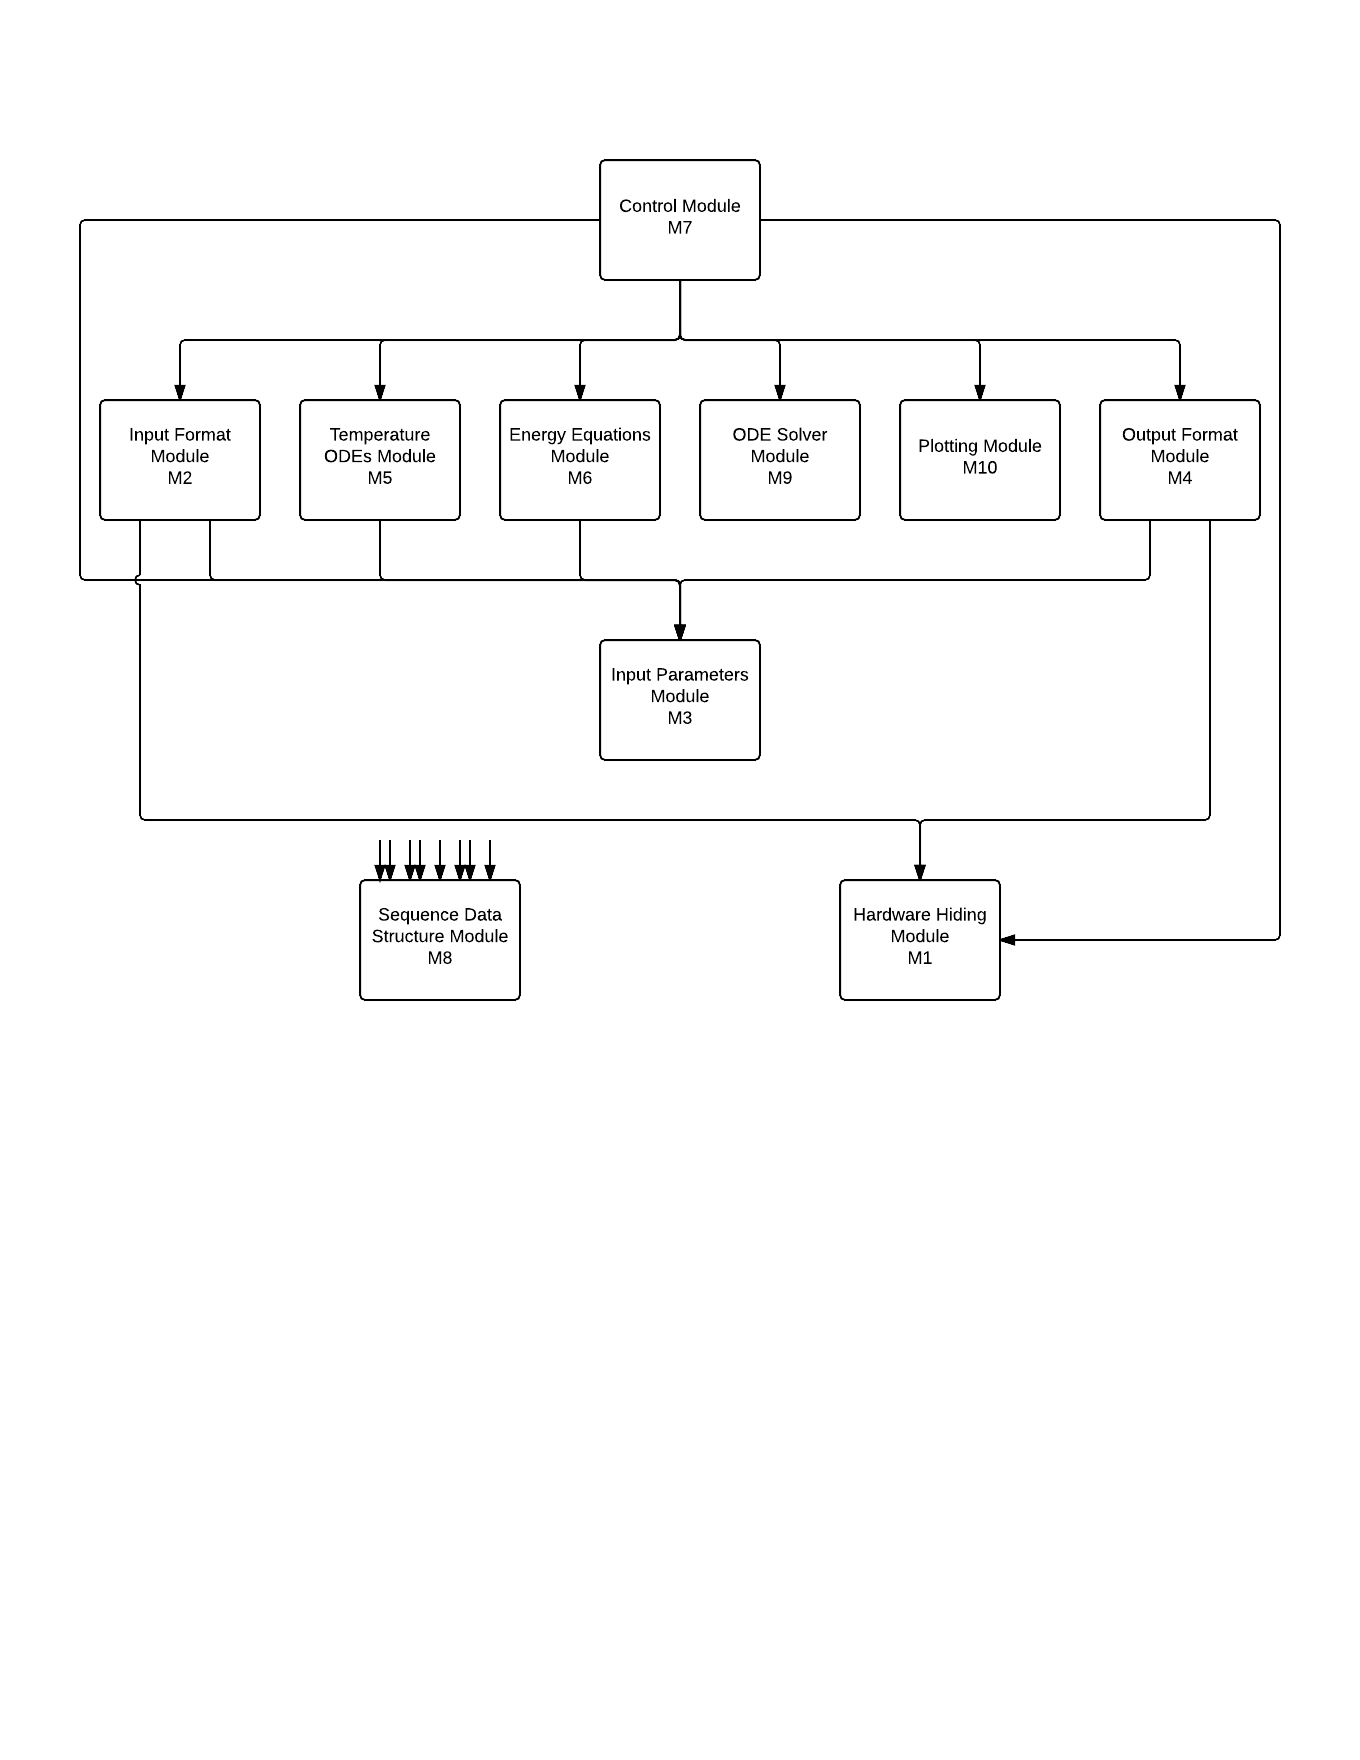
\includegraphics[width=0.7\textwidth]{UsesHierarchy.png}
\caption{Use Hierarchy among Modules}
\label{FigUH}
\end{figure}

%\section*{References}

\bibliographystyle {plainnat}
\bibliography {../SRS/PCM_SRS}

\end{document}
